\label{sec:2.3}
%%%%%%%%%%%%%%%%%%%%%%%%%%%%%%%%%%%%%%%%%%%%%%%%%%%%%%%
%(Christian) Fermilab test setup including the test boards
%%%%%%%%%%%%%%%%%%%%%%%%%%%%%%%%%%%%%%%%%%%%%%%%%%%%%%%
\begin{figure}[htb]
\centering
%\begin{minipage}[b]{1.0\textwidth}
\begin{center}
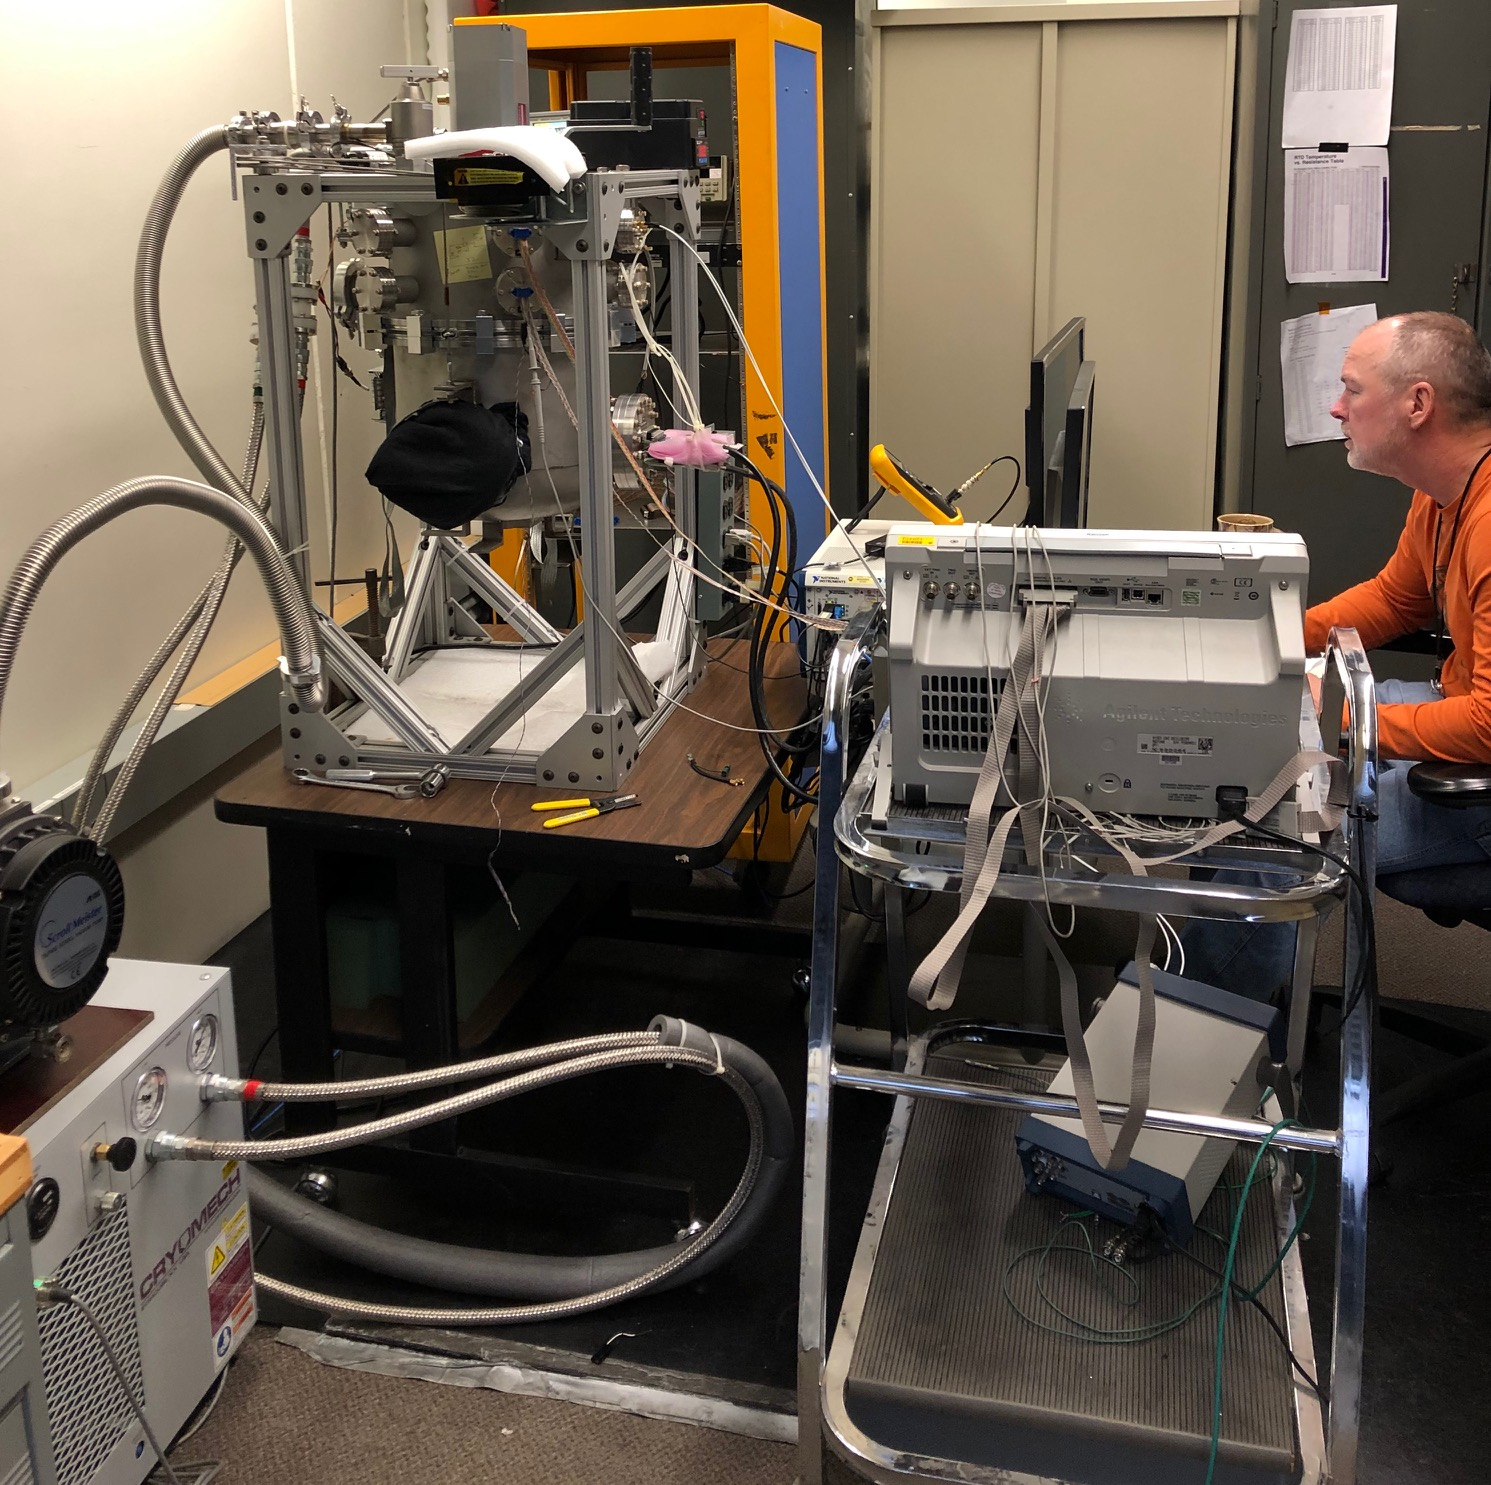
\includegraphics[width=0.95\textwidth]{figures/cryotestsystem.jpg}
\end{center}
%\end{minipage}
\caption{Fermilab Cryocooler Test System.}
\label{fig:cryocoolertestsystem}
\end{figure}

The Fermilab Cryocooler Test System consists of a vacuum vessel and a cryogenic refrigerator. The cryogenic refrigerator is a Cryomech PT-60.  It is a closed-loop cryocooler consisting of a helium compressor (located next to the vacuum vessel) and a cold head (located on top of the vacuum vessel).  The cryocooler cools a copper cold-plate inside the vacuum vessel to a minimum of 60 K.  A 100 ohm platinum RTD and a 75 Watt heater are mounted on the cold-plate.  A temperature controller cycles the heater on and off to achieve the set-point temperature.  Any temperature between 60 and 250 K can be set.
The vacuum vessel has 2 large penetrations and 12 small penetrations that can be used in device testing.  Typically, one of the large penetrations is used as an inspection port and the other as a feedthrough for ribbon cables.  The small ports allow for a variety of other signal feedthroughs.  

Two printed circuit boards are used in ASIC testing, a ``cold board,'' which is screwed onto the cold-plate and includes a large unmasked copper thermal contact area, and a ``warm board'' which is mounted as a mezzanine board on the cold-board.  RTDs are placed on both the cold board and the warm board.  The temperature on the warm board is typically 100 K higher than than the temperature on the cold board.  If the cryocooler is regulated to hold the cold-board at LN$_2$ temperature, then the temperature on the warm board is $\sim-96^{\circ}$C, which is warm enough for most COTS components to operate properly.

The cold board used in tests of COLDADC includes a single bare chip, wire bonded to the printed circuit board.  An 80-pin header carries digital I/O and three of the four bias voltages (VDDIO and both digital voltages) between the cold board and the warm board.  A 60 pin header carries the analog bias voltage and all analog signals with the exception of the analog inputs to the COLDADC.  Jumpers allow the analog inputs to be grounded or connected to an external sources using cables.  The only other parts on the cold board are bypass capacitors (selected for cryogenic use) and test points.

The warm board includes connectors that mate to the cold board connectors, a 52-pin header used for a cable connection to an National Instruments (NI) FPGA module, single ended to differential converters used for the 64 and 2 MHz clock signals, differential to single ended converters for the LVDS output signals, level shifters for the CMOS I/O signals, passive components, buffer amplifiers, and SMA connectors for the analog outputs, SMA connectors for the ADC test inputs, and 9-pin D connectors for cable connections to NI power supplies that provide source-measure functionality (used for chip power and for providing or measuring analog I/O signals such as reference voltages).

Test software was written using National Instruments LabView and run on a single-crate PXIe system consisting of a controller, an NI 6583 FPGA unit, and 5 power supply modules.  A Keysight 33500B waveform generator was used to provide input signals.  Analog measurements were made using an oscilloscope and a DVM as well as with the NI modules.

